\documentclass{standalone}
\usepackage{tikz}
\usepackage{amsmath,amssymb}
%\usetikzlibrary{fpu}
\begin{document}
	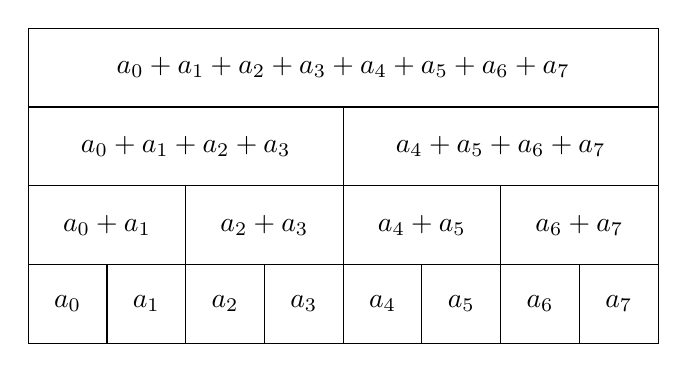
\begin{tikzpicture}
		\draw (0,0) rectangle (8,-4);
		\foreach \i in {-1,-2,-3}{
			\draw (0,\i) -- (8,\i);
		}
		\foreach \i in {4}{
			\draw (\i,-1) -- (\i,-2);
		}
		\foreach \i in {2,4,6}{
			\draw (\i,-2) -- (\i,-3);
		}
		\foreach \i in {1,2,...,7}{
			\draw (\i,-3) -- (\i,-4);
		}
		\foreach \i in {0,1,...,7}{
			\node at (\i+0.5,-3.5) {$ a_{\i} $};
		}
		\foreach \i in {0,2,4,6}{
			\pgfmathsetmacro{\x}{int(\i+1)}
			\node at (\i+1, -2.5) {$ a_{\i}+a_{\x} $};
		}
		\foreach \i in {0,4}{
			\pgfmathsetmacro{\x}{int(\i+1)}
			\pgfmathsetmacro{\y}{int(\i+2)}
			\pgfmathsetmacro{\z}{int(\i+3)}
			\node at (\i+2, -1.5) {$ a_{\i}+a_{\x}+a_{\y}+a_{\z} $};
		}
		\foreach \i in {0}{
			\node at (\i+4,-0.5) {$ a_{0}+a_{1}+a_{2}+a_{3}+a_{4}+a_{5}+a_{6}+a_{7} $};
		}
	\end{tikzpicture}
\end{document}